\label{sec:ProtokolDesign}
\todo{alle bilder mit caption und label!!!}
Dieses Kapitel soll einen Überlick über das eigentliche Design des Content
Relevant-Oriented Protocol (CROP) geben und indes auf den Aufbau und die
Strukturierung der zu sendenden Nachricht eingehen.\todo{anderen anfang - so
fängt hier jeder absatz an\ldots !!}

Zentrale Rolle spielte dabei der Header der Nachricht. Dieser beinhaltet
Informationen, die zum eindeutigen Versenden und Identifizieren der
mitgelieferten Daten notwendig sind. Dazu gehören zum Einen die Versionsnummer,
die Konfiguration und die Länge der Nachricht, zum Anderen die genauen Adressen
des Senders und Empfängers. Neben dem Header sind die verpackten Daten, der
sogenannte Payload, und ein CRC-Code zur Fehlerüberprüfung der Nachricht
vorhanden. In Abbildung \ref{fig:DatenaufschluesselungMessage} ist der Header
einer Nachricht im Detail dargestellt.

\begin{figure}[H]
	\centering
	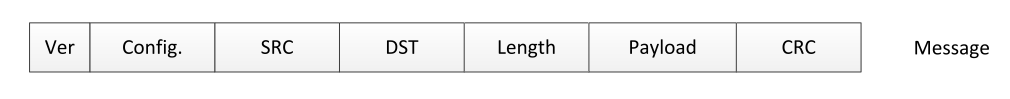
\includegraphics[width=\textwidth]{DatenaufschluesselungMessage.png}
	\caption{Datenaufschlüsselung der Nachricht}
	\label{fig:DatenaufschluesselungMessage}
\end{figure}

Die Versionsnummer belegt die ersten vier Bits des Headers. Diese
signalisiert dem Empfänger mit welcher Version des Protokolls die Nachricht
verpackt und versand wurde. Darauf folgt die Konfiguration. Mit Hilfe dieser,
können Einstellungen vorgenommen werden, welche die Größe der gesamten Nachricht
beeinflussen. Somit ist in speziellen Fällen eine schnellere Übertragung der
Nachricht möglich, da keine überflüssigen Informationen oder Bits vorhanden
sind. Für die Konfiguration wurden $12$ Bits reserviert. Die ersten drei Bits
bestimmen das Adressformat. Diese ermöglichen das Aufsetzen des Protokolls auf
bereits bestehenden Standards, wie IPv6 oder des Bundle-Protokolls.
Die verbleibenden neun Bits sind reserviert und dienen zur Erweiterung des
Protokolls für zusätzliche Einstellungsmöglichkeiten. Die Bitvergabe
der Adressen von Sender und Empfänger erfolgt dynamisch abhängig der
Konfiguration.
Dies ist für die Nutzung unterschiedlicher Übertragungsprotkolle notwendig.
Für IPv6 werden $128$ Bit bereitgestellt. dies sind jeweils $64$ Bit für
die Sender- und Empfängeradresse. Die Länge repräsentiert die Größe der gesamten
Nachricht in Bytes und belegt die nächsten $24$ Bit.
Der vorletzte Bestandteil der Nachricht, der sogenannte Payload, beinhaltet die
eigentlich Daten und besteht aus mehreren Datenblöcken. Am Ende werden noch
die Püfsummenbits zur Fehlererkennung hinzugefügt. Diese sind $16$ Bits lang,
wenn die Gesamtlänge der Nachricht kleiner gleich $2^{16}$ Byte beträgt.
Anderfalls beträgt die Länge $32$ Bits. Durch diese Unterteilung kann
Overhead vermieden werden und trotzdem ist gewährleistet große Nachrichten
verschicken zu können.

\begin{figure}[H]
	\centering
	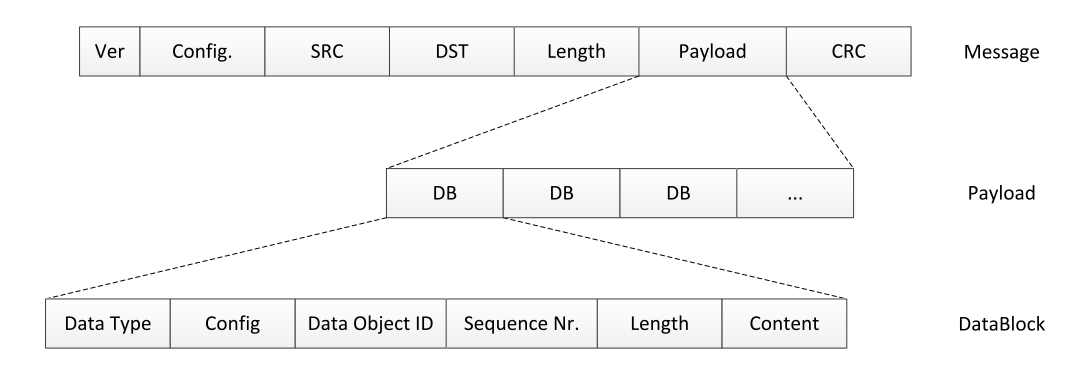
\includegraphics[width=\textwidth]{DatenaufschluesselungDB.png}
	\caption{Aufschlüsselung der Datenblöcke}
  \label{fig:DatenaufschluesselungDB}
\end{figure}

Ein Datenblock besteht aus den folgenden Teilen: DOID (Data Object
Identification Number), Datentyp, Config, Sequenznummer und der Länge des Datenblocks. Die DOID
repräsentiert die Datei (Bild, Text, Sensorwerte,\ldots) dem der Datenblock
angehört. Das Differenzieren der einzelnen Datenblöcke untereinander erfolgt
mittels der Sequenznummer. Das Einführen des Datentyps im Header ermöglichte
noch mehr unterschiedliche Datenblöcke, da DOID und Sequenznummer nur einem
Datentyp zugeordnet werden.
Innerhalb des Datentypes geben die ersten $4$ Bits den übergeordneten Typ (Bild,
Text, \ldots) an und die Verbleibenden spezifizieren das genaue Format (jpg, txt, \ldots).
Die Config beträgt $6$ Bits. Dabei sind die vordersten drei Bits die Kompression
des Datenblockheaders, damit kann die Längen der DOID, der SequenzNummer und
der Länge des gesamten Datenblockes varriert und somit Overhead gespart werden.
Das vierte Bit gibt an, ob ein Zeitstempel nach dem Header von $8$
Byte gesetzt wird.
\todo{reihenfolge wäre das nicht besser vor den fertigen Datenblock header??
also weg vor ziel und nicht ziel vor weg ;)} Eine schnelle und eindeutige
Zuordnung eines einzelnen Datenblockes auf der Empfängerseite, stand bei der Entwicklung des Headers im Mittelpunkt. Das heißt
neben der Bitvergabe war eine genaue Überlegung über die richtige Reihenfolge
notwendig. Hierzu gibt es die in Abbildung dargestellten drei Ansätze.

\begin{figure}[H]
	\centering
	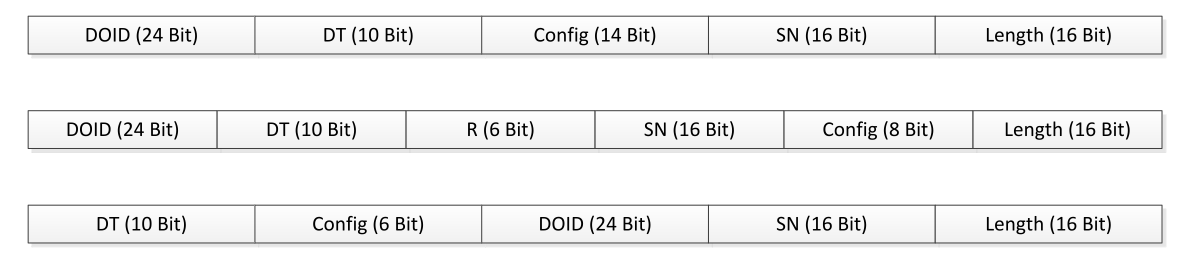
\includegraphics[width=\textwidth]{DatenblockVarianten.png}
\end{figure}

Ausgegangen wurde anfangs von je acht Bit für Datentyp und Config. Dabei kam die
Frage auf, ob diese wirklich ausreichen, da sehr viele verschiedene Datentypen
und Formate existieren. Infolgedessen wurde, wie in Variante $1$ zu sehen, ein
zusätzliches Byte zur Verfügung gestellt. Aufgeteilt zu zwei Bit für den
Datentyp und sechs Bit für die Config. Dieser Variante lag die Idee zu Grunde,
dass der Datenblock als erstes über die DOID und im folgenden dem ihm
zugeordneten Datentyp identifiziert wird. Folgen sollte die Config und
anschließend die Sequenznummer. Ein ähnlicher Ablauf galt auch für Möglichkeit
$2$, bei der die restlichen sechs Bit zur Vorreservierung größerer Datentypen
genutzt wurden. Dies war bezüglich des Datentyps und der Menge unterschiedlicher
Datenblöcke die bessere Variante. \todo{müssen wir nochmal genau schauen da bin
ich mir gerade iwi net sicher wie das genau war!!!} Als effektivste Maßnahme
ergab sich am Ende aber nicht aus dem Spendieren eines zusätzlichen Bytes,
sondern die Reihenfolge in der die Bestandteile im Header angeordnet sind. Wie
in Variante $3$ ersichtlich, wurden sechs Bit gespart, die Anrodnung aber derart
verändert, dass ein Datenblock zunächst an seinem Datentyp identifiziert wird.
Dies ist sinnvoller, da sofort eine Eingrenzung der möglichen Daten-Objekte
(DOIDs) eintritt. Erst dann folgt die DOID und die Sequenznummer. Die Config
an zweiter Stelle ermöglicht einen schnellen Überblick über eventuelle
Einstellungen des Headers. So existiert neben den Kompressionsmöglichkeiten ein
weiteres Bit in der Config, das einen sogenannten Timestamp aktiviert. Dieser
repräsentiert die Zeit, zu dem die Daten des Datenblocks aufgenommen wurden. Das
Timestamp-Flag in der Config wurde eingeführt, um einen Overhead bei
beispielsweise Texten oder Bildern zu vermeiden. Die Idee besteht darin, dass
auf Grund der geringen größe einzelner Sensordaten und dem darausfolgenden
Overhead beim Verschicken, mehrere Sensordaten in einem Datenblock
zusammengefasst werden. Da jeder dieser Sensordaten zu einem anderen Zeitpunkt
aufgenommen wurde, ist für diese ein seperater Timestamp notwendig (siehe Bild
LETZTE GEILE AUFSPLITTUNG), anders als bei Bildern oder Texten. 

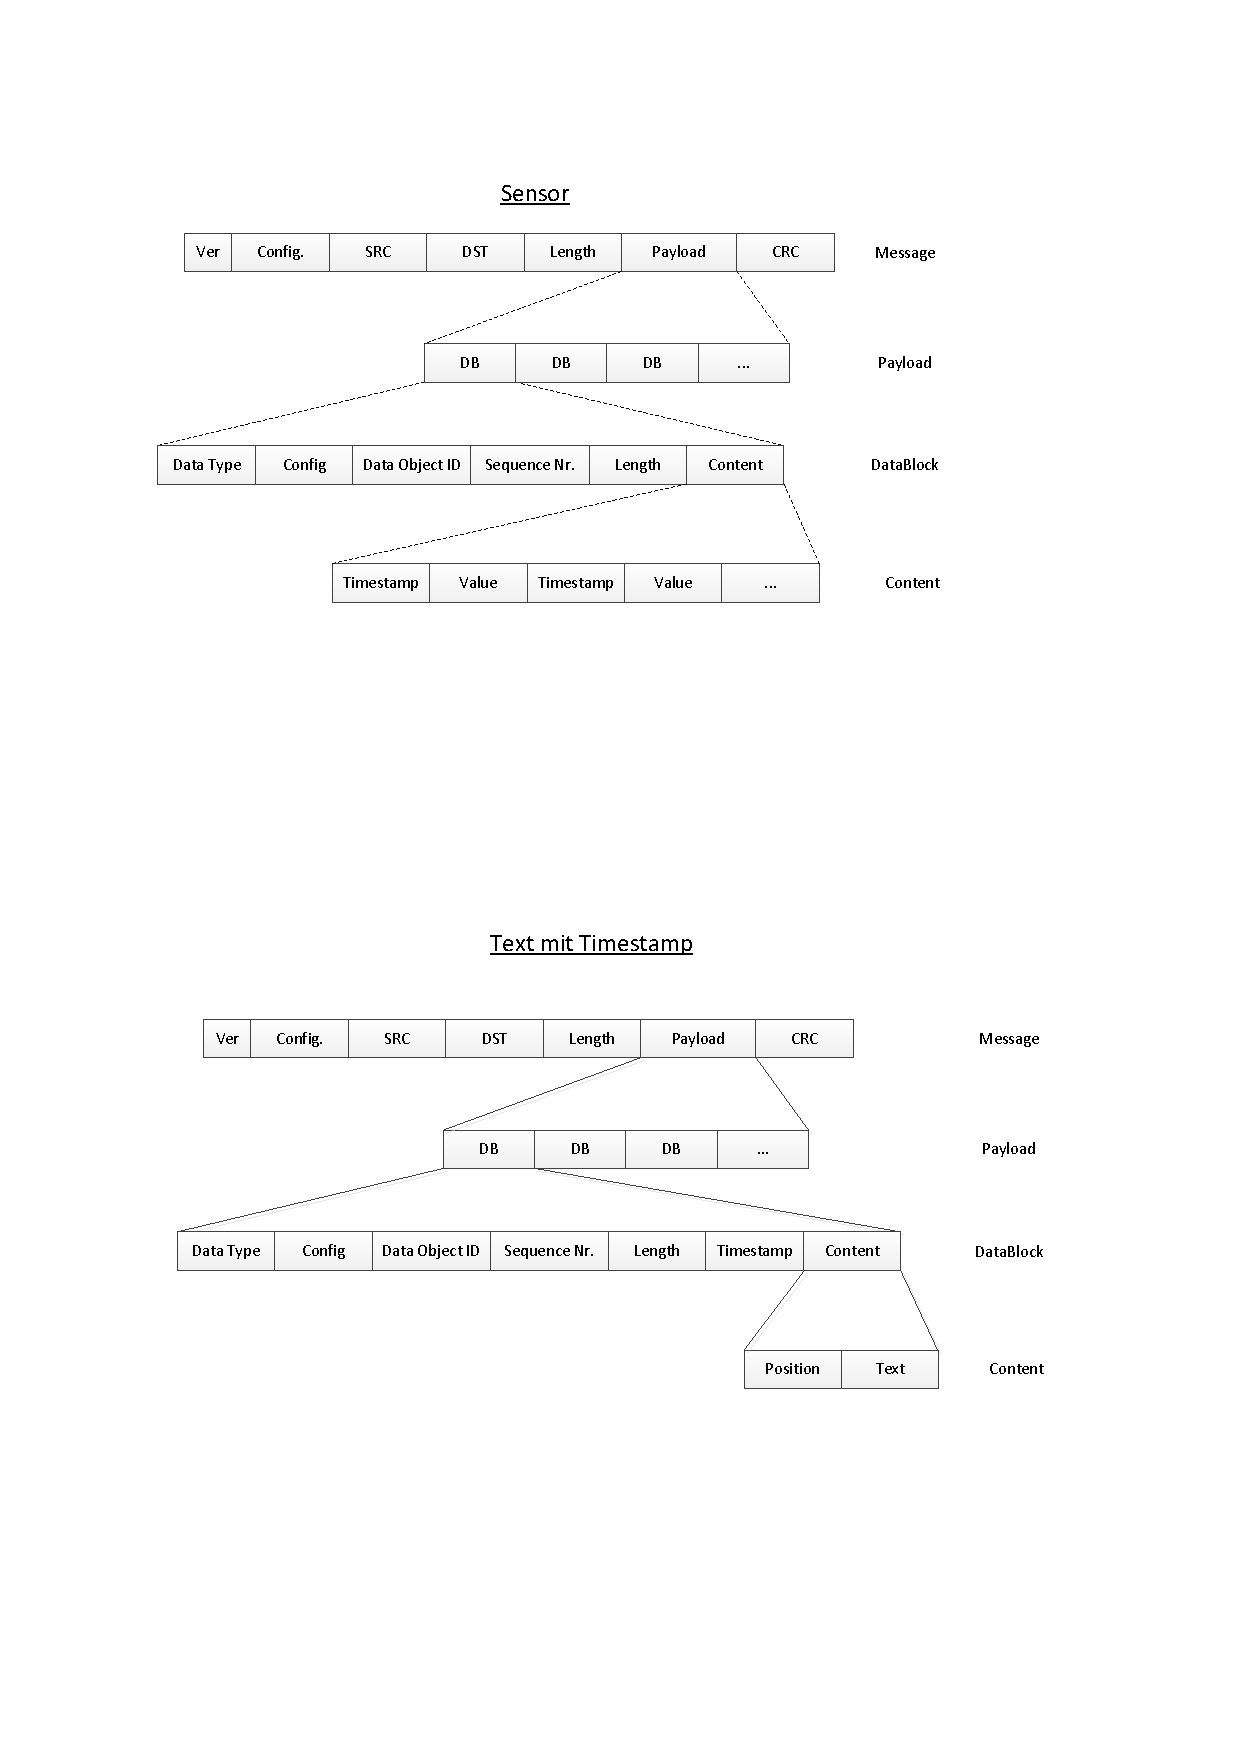
\includepdf{Datenaufschluesselung.pdf}

Das Bild \ref{fig:beispielJPG} zeigt die beispielhafte Aufsplittung noch einmal
an Hand JPEG Bildes. Wie zu erkennen, besteht das Bild aus mehreren "Contents"
die wiederum eine vielzahl an Pixeln vereinen (siehe "Gesplittetes JPEG" im
Bild). Diese Bildaten in Verbindung mit dem "JPEG-Header" bilden den gesamten
Content. Ein Datenblock besteht dann wie oben beschrieben und im Bild
\ref{fig:beispielJPG} (rechter Teil) zu sehen aus diesem Content und dem
dazugehörigen Datenblockheader.

\begin{figure}[H]
	\centering
	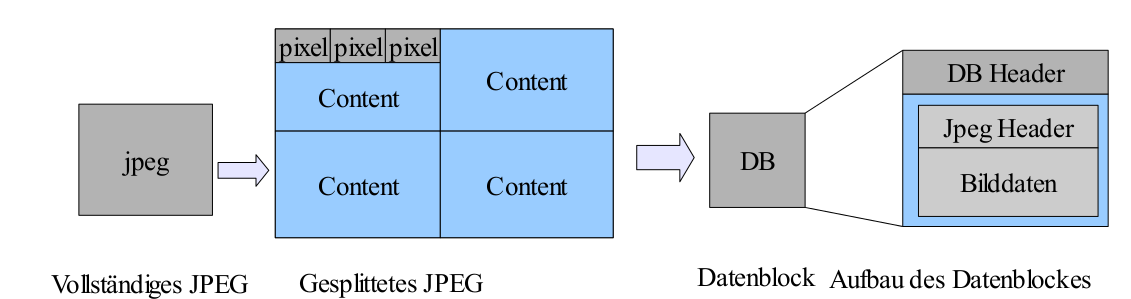
\includegraphics[width=\textwidth]{beispielMessage.png}
	\label{fig:beispielJPG}
\end{figure}

Neben der Strukturierung und des Aufbaus der Nachricht selbst ist auch die
Priorisierung einzelner Datenblöcke sehr wichtig. Also in welcher Reihenfolge
Nachrichten versandt werden. Die Priorisierung erfolgt hierbei grundlegend in
zwei Schritten, wie Bild \ref{fig:priorisierungen} zeigt. Zunächst erfolgt eine
Art Vorpriorisierung. Dabei werden relevantere Bereiche selektiert und durch den
sogenannten "relevance Value" höher eingestuft. Die Datei wird daraufhin je nach
definierten Regeln in einzelne Datenblöcke eingeteilt (siehe Bild
\ref{fig:priorisierungen} rechts). Diese erhalten je nach Wichtigkeit eine
Priorisierung ("prio Value"). Datenblöcke relevanter Bereiche werden, nach ihrem
Informationsgehalt, extra priorisiert. Dabei wird davon ausgegangen, wieviel
Anteile des Datenblocks (in Prozent) wichtigen Inhalt, das heißt einen
entsprechenden Teil des relevanten Objektes, enthalten. Nach der Priorisierung
erfolgt eine Einsortierung der Datenblöcke unter Berücksichtigung des "relevance
Value" und "prio value" in die "Prioritization-Queue" (siehe Abschnitt
\todo{label zum abschnitt über die prio queue}). 

\begin{figure}[H]
	\centering
	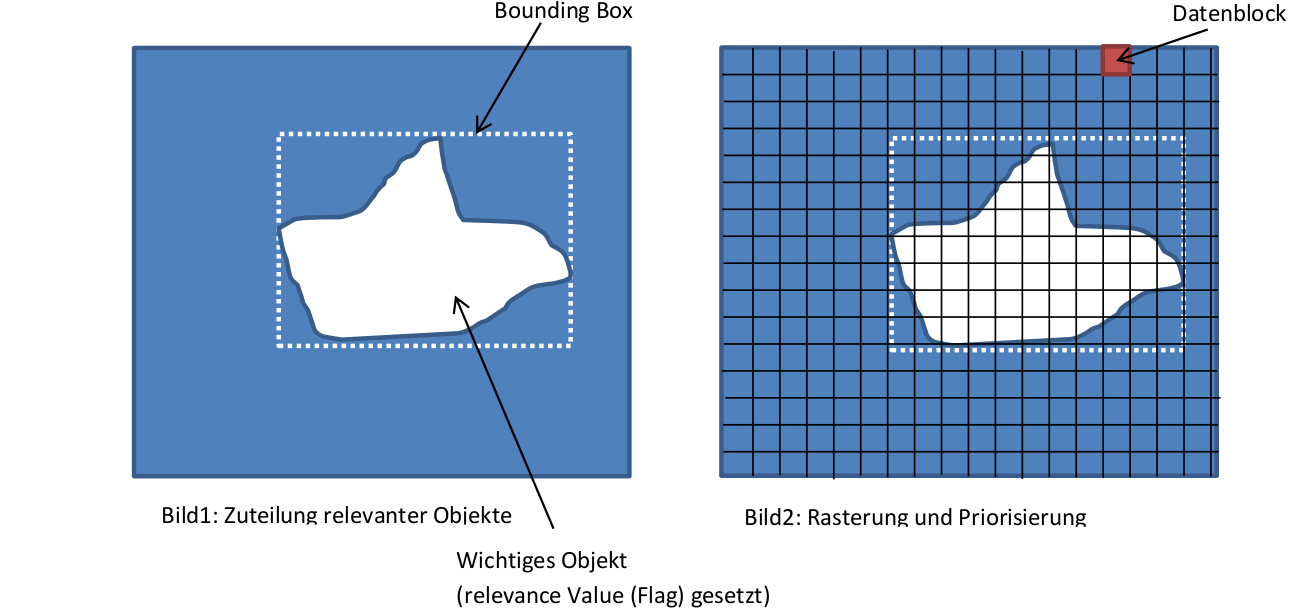
\includegraphics[width=\textwidth]{Priorisierung.png}
	\label{fig:priorisierungen}
\end{figure}
